\section{Discretization limit at very small \texorpdfstring{$p$}{p}}\label{app:smallp}

Figure~\ref{fig:smallp} shows the gain on D2 down to $p=10^{-7}$ and the diagnostic variants. Two alternative explanations of the breakdown below $p=10^{-5}$ were ruled out. Lowering the step floor of the splitting chains tenfold, or removing it, leaves every run unchanged: the floor is never reached. An additional move that redraws a random subset of coordinates from the uniform distribution, akin to the componentwise Metropolis algorithm of the original subset simulation~\cite{AuBeck2001}, helps only partly: at $p=10^{-6}$, splitting then succeeds in 50\% of runs and the portfolio in 68\%, but at $10^{-7}$, there is still no gain. The same move doubles the gain at $p=10^{-4}$ (53 for splitting and 35 for the portfolio); it is a natural extension of the method but is not used elsewhere in this paper. Reducing the integration step restores the order-of-growth gain, as stated in section~\ref{sec:scaling_p}. These gains are counted in integrations, each of which is 4 or 16 times longer, so the gain in computing time is correspondingly smaller; the test demonstrates the mechanism, not a practical speedup. The level threshold also explains why one informative point is not enough. The level $\xi_l$ is the tenth largest value in the reference sample; when fewer than ten points are informative, the threshold is $\xi_l=0$ (all escapes at the first step tie), the level cannot rise, and the chains stagnate and restart. The gain at $p=10^{-5}$ is carried by the runs whose reference sample contains several informative points. Figure~\ref{fig:scaln} shows the dependence on dimension at fixed $p=10^{-4}$.

\begin{figure}[tbhp]
\centering
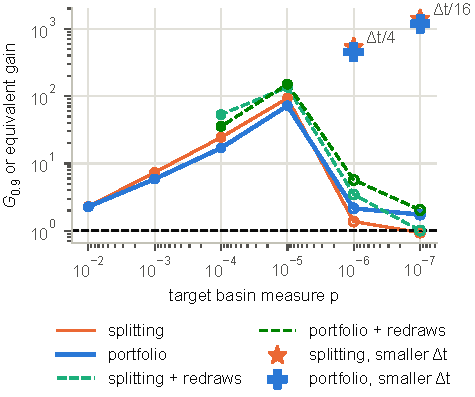
\includegraphics[width=0.62\textwidth]{figures/fig29_d2_small_p.pdf}
\caption{Family D2 ($n=6$): gain down to $p=10^{-7}$. Filled markers: $G_{0.9}$; open markers: the equivalent gain $-\ln(1-f)/(pN_{\max})$ from the fraction $f$ of runs that found the target within the budget $N_{\max}$. Dashed lines: the variant with an additional move that redraws a random subset of coordinates (the variants with a lowered step floor coincide with the base curves and are not shown). Stars and crosses: splitting and the portfolio with the integration step reduced 4 times ($p=10^{-6}$) and 16 times ($p=10^{-7}$), with $N^0_{0.9}=\ln10/p$.}
\label{fig:smallp}
\end{figure}

\begin{figure}[tbhp]
\centering
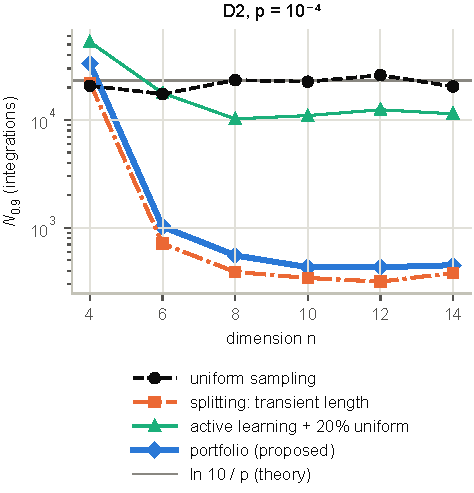
\includegraphics[width=0.62\textwidth]{figures/fig24_scaling_n.pdf}
\caption{Detection cost versus the phase-space dimension (family D2, $p=10^{-4}$, $R=100$). Thin gray line: $\ln10/p$. At $n=4$, the reaction coordinate is uninformative because of the discretization limit; for $n\ge6$, the portfolio gains 17--61.}
\label{fig:scaln}
\end{figure}

